\mySection{System Overview}
Our system's primary goal is to help school faculties perform roll calls with ease.
Traditional roll calls require teachers to call the names of students individually to record students' attendance,
while PyRollCall let a teacher simply take a photo of the entire class and record students' attendance
using Facial Recognition, thus saving more time for both teachers and students in classes.
\vspace{0.5cm}

Another usage of this system is taking the photo of each student one by one as long as
the size of the class is small enough. If the size of the class is too large, this apparently
can result in longer waiting time for the students, and hence this approach is impractical.
Consequently, our main objective is to ensure that the system can accurately recognize all the faces
in a large image as possible as it can.
\vspace{0.5cm}

PyRollCall is able to run on Windows, macOS and unix-like systems as long as the system supports
Python 3 and running GUI applications. Figure~\ref{fig:systemAppearance} demonstrates the appearance
of this system. The actions that can be performed using the GUI are listed as follows:
\vspace{0.5cm}

\setstretch{0.8}
\begin{itemize}
  \item Maintain the data of the course and students they teach.
  \item Take photos of students with a camera and train the neural network.
  \item Perform roll calls.
  \item Export the result of roll calls to files.
\end{itemize}
\setstretch{\myContentLineSpacing}

\begin{figure}[!htb]
  \centering
  \begin{subfigure}[b]{0.32\linewidth}
    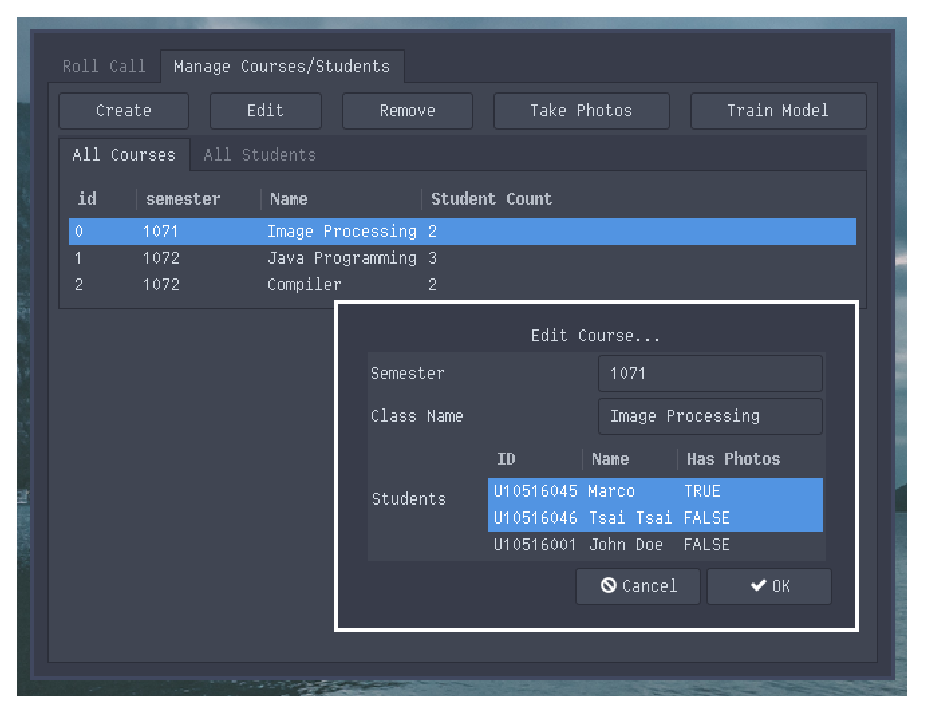
\includegraphics[width=\linewidth]{figures/preview1.eps}
    \caption{Managing courses.}
  \end{subfigure}
  \begin{subfigure}[b]{0.32\linewidth}
    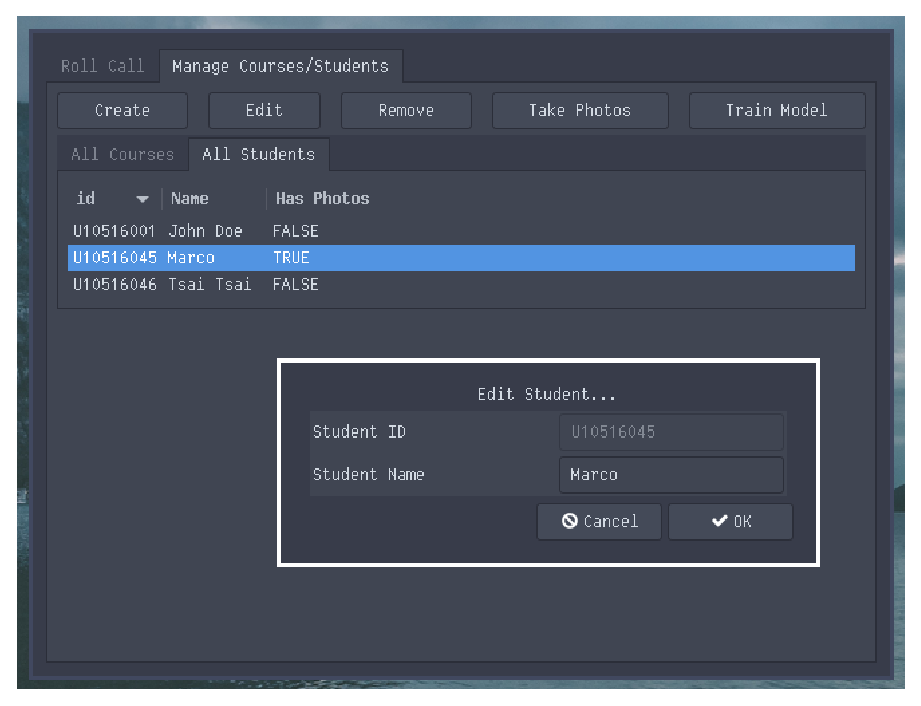
\includegraphics[width=\linewidth]{figures/preview2.eps}
    \caption{Managing students.}
  \end{subfigure}
  \begin{subfigure}[b]{0.32\linewidth}
    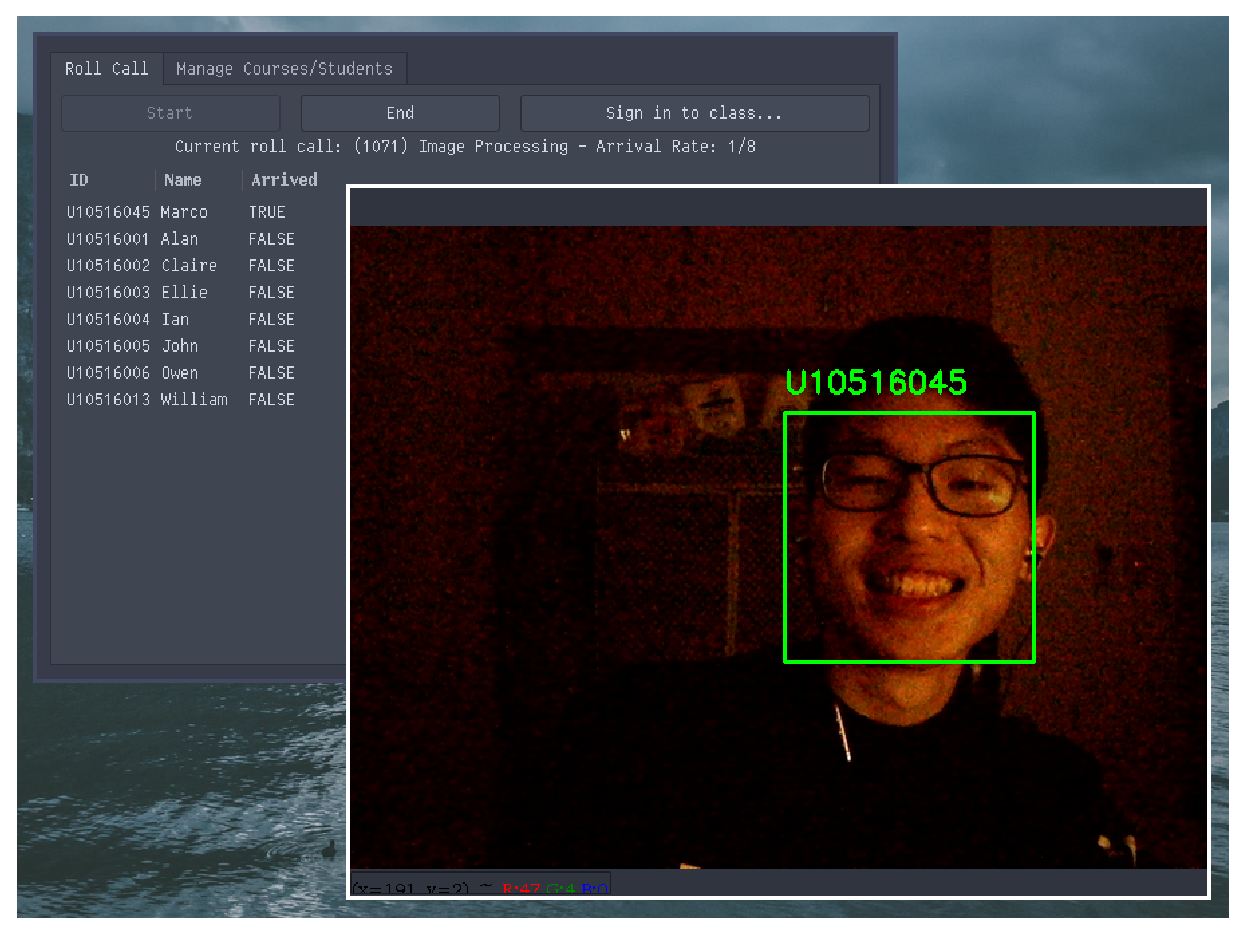
\includegraphics[width=\linewidth]{figures/preview3.eps}
    \caption{A student signing in.}
  \end{subfigure}
  \caption{PyRollCall running on a Linux machine with X11\protect\footnotemark \ installed.}
  \label{fig:systemAppearance}
\end{figure}

\footnotetext{X11, also known as X Window System, or simply X, is a windowing system that provides the basic framework for building GUI environments.}


\subsection{Getting Started}
The remainder of this section is dedicated to documenting the process to checkout and
execute PyRollCall. To ensure that a copy of the project can be properly obtained and
run, please make sure the following tools are accessible on your system:
\vspace{0.5cm}

\setstretch{0.8}
\begin{itemize}
  \item A system environment which supports GUI applications
  \item Python 3 (preferably Python 3.5+)
  \item Git
 \end{itemize}
\setstretch{\myContentLineSpacing}

Windows and macOS should natively support GUI applications. However, if you are running Linux,
some distributions such as CentOS, Arch and Gentoo might not, by default, support
GUI applications. In this case, you'll have to manually install X11 packages on your system.

\subsection{Installation}
PyRollCall is open-sourced and managed with \emph{git}\footnote{git is a distributed version control system used for tracking file\
  content changes in source code during software development}. All of its external dependencies are already packaged
in the project via Python's {virtualenv}\footnote{virtualenv is a tool to created isolated Python environments by maintaining a set of libraries that a specific application depends on.},
thus the users do not have to worry about what and which versions of libraries they need to install. To checkout and run the project:

\begin{lstlisting}[numbers=none,xleftmargin=0em,caption={Shell commands to checkout and run PyRollCall}]
$ git clone https://github.com/aesophor/pyrollcall.git
$ cd pyrollcall
$ source venv/bin/activate
$ ./pyrollcall.py 
\end{lstlisting}

The entry point to the system is the script \emph{pyrollcall.py}, a script located under the project's root directory.
Before executing it, source the shell script \emph{venv/bin/activate} to activate the project's virtual environment.
